\begin{pregunta}
\puntaje{5}
\begin{cuerpo}
La gráfica 
\begin{center}
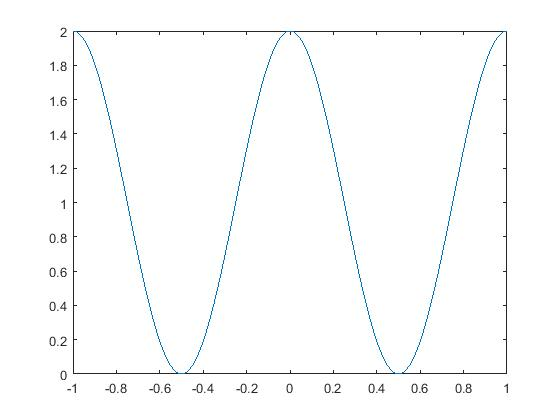
\includegraphics[width=0.5\textwidth]{./img/img1.jpg}
\end{center}
se genera con las instrucciones
\end{cuerpo}
\begin{multicols}{2}
\begin{alternativas}
{\texttt{
x=-1:0.01:1; \\
y=cos(2*pi*x)+1; \\
plot(x,y);}}
{\texttt{
x=-1:0.01:1; \\
y=cos(2*pi*x); \\
plot(x,y);}\\} 
{\texttt{
x=-1:0.01:1; \\
y=sin(2*pi*x)+1; \\
plot(x,y);}}
{\texttt{
plot(cos(x)+1);}}
\end{alternativas}
os\end{multicols}
\justificacion{0cm}
\end{pregunta}